\documentclass[10pt]{article}
\usepackage[margin=1in]{geometry}

\usepackage{biblatex}
\addbibresource{./references.bib}

\usepackage{hyperref}
\usepackage{xcolor}
\hypersetup{
    colorlinks,
    linkcolor={red!70!black},
    citecolor={blue!70!black},
    urlcolor={blue!90!black}
}

\usepackage{tikz}
\usetikzlibrary{shapes,arrows}
\usetikzlibrary{arrows.meta}
\usetikzlibrary{shapes.multipart}

\begin{document}
This is an overview of the material point method.
While there are many variants due to the experimental nature of MPM, this document is focused on the current implementation.
For a more general review, please see the paper by \textcite{buzzi08}.

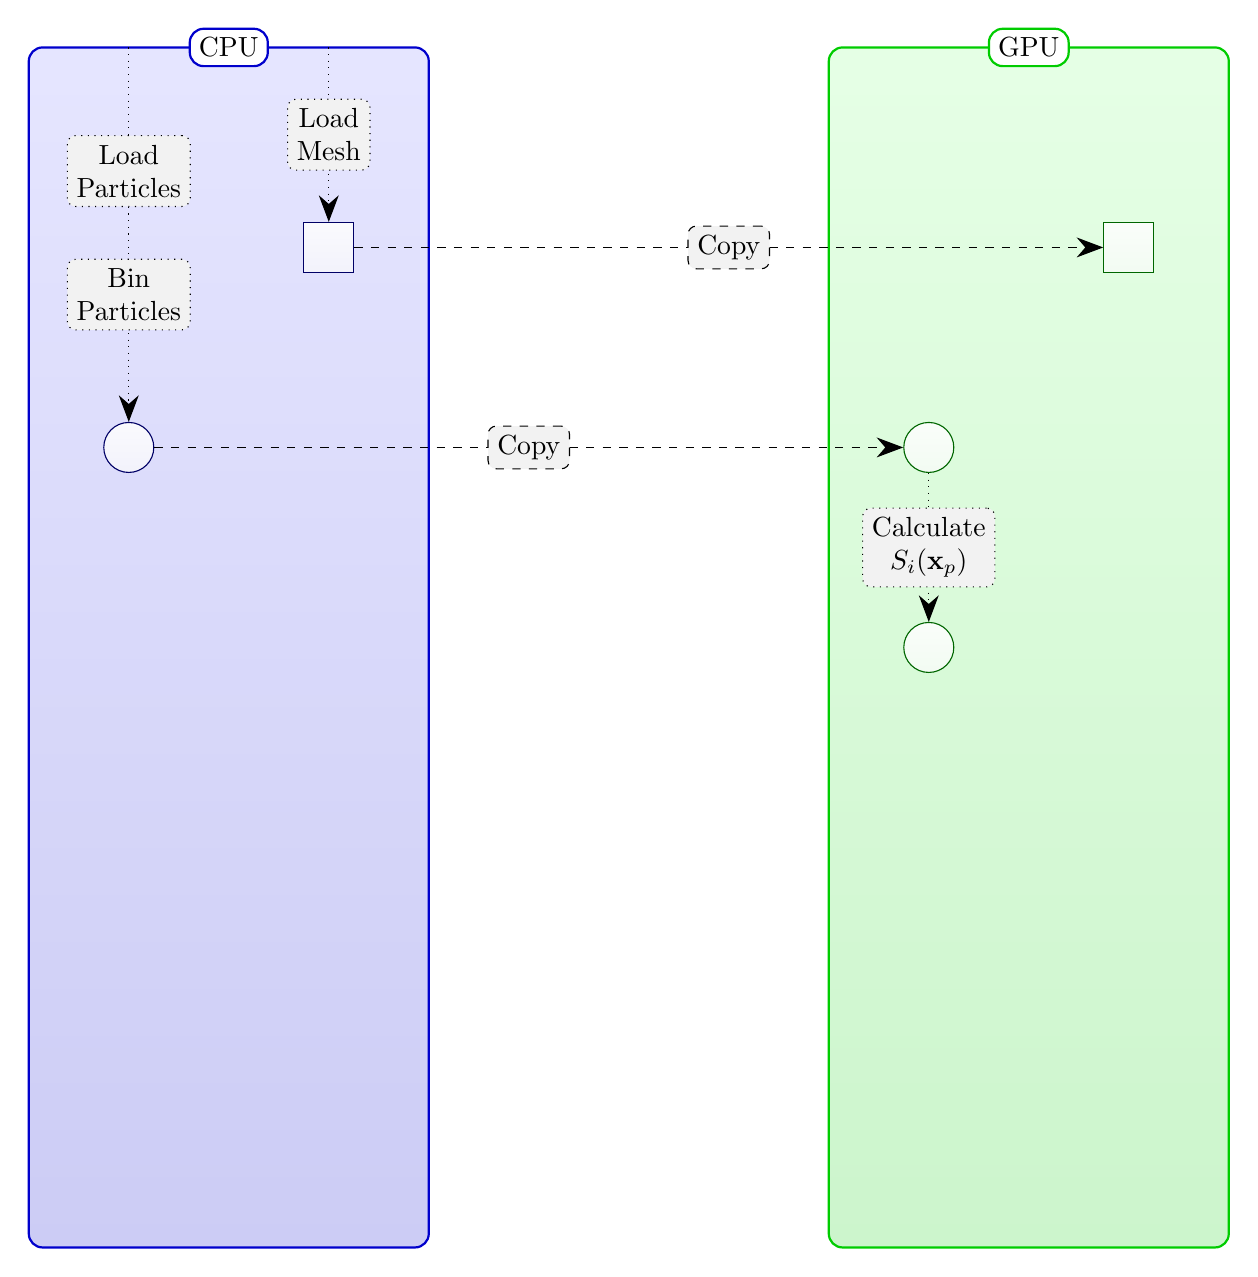
\begin{tikzpicture}
\tikzstyle{gpuborder}=[thick, draw=green!80!black]
\tikzstyle{gpushade}=[shade, top color=green!10, bottom color=green!80!black!20]
\tikzstyle{ongpu}=[draw=green!40!black, shade, top color=green!70!black!2, bottom color=green!70!black!5]
\tikzstyle{cpuborder}=[thick, draw=blue!80!black]
\tikzstyle{cpushade}=[shade, top color=blue!10, bottom color=blue!80!black!20]
\tikzstyle{oncpu}=[draw=blue!40!black, shade, top color=blue!70!black!2, bottom color=blue!70!black!5]
\tikzstyle{copy}=[draw=black,dashed,-{Stealth[scale=2]}]
\tikzstyle{function}=[draw=black,dotted,-{Stealth[scale=2]}]
\tikzstyle{functionbox}=[rounded corners=3pt, draw=black, fill=black!5, align=center]
\tikzstyle{ms}=[minimum size=0.25in]
\tikzstyle{mesh}=[ms]
\tikzstyle{particle}=[ms, circle]

% Background 'containers'
\path[cpushade, cpuborder, rounded corners=5pt] (0, 0) -- (0, 6in) -- (2in, 6in) node[pos=0.5, fill=white, cpuborder] {CPU} -- (2in, 0) -- cycle;
\path[gpushade, gpuborder, rounded corners=5pt] (4in, 0) -- (4in, 6in) -- (6in, 6in) node[pos=0.5, fill=white, gpuborder] {GPU} -- (6in, 0) -- cycle;

\coordinate (start-particle) at (0.5in, 6in);
\coordinate (start-mesh) at (1.5in, 6in);

\node[oncpu, particle] (init-pstate) at (0.5in, 4in) {};
\node[oncpu, mesh] (init-mstate) at (1.5in, 5in) {};

\node[ongpu, particle] (gpu-init-pstate) at (4.5in, 4in) {};
\node[ongpu, particle] (gpu-sf-pstate) at (4.5in, 3in) {};
\node[ongpu, mesh] (gpu-init-mstate) at (5.5in, 5in) {};

\path[copy] (init-pstate) -- (gpu-init-pstate) node[functionbox, pos=0.5] {Copy};
\path[copy] (init-mstate) -- (gpu-init-mstate) node[functionbox, pos=0.5] {Copy};

\path[function] (start-particle) -- (init-pstate) node[functionbox, pos=0.33] {Load \\ Particles} node[functionbox, pos=0.66] {Bin \\ Particles};
\path[function] (start-mesh) -- (init-mstate) node[functionbox, pos=0.5] {Load \\ Mesh};

\path[function] (gpu-init-pstate) -- (gpu-sf-pstate) node[functionbox, pos=0.5] {Calculate \\ $S_i(\mathbf{x}_p)$};
\end{tikzpicture}

The inital sorting of material points is done by the GPU, checking the particles against every element.
For subsequent sortings, we use coherence, which means that particles most often will stay within the same element or move at most one element away during a time step.

After sorting the particles into elements, we then compute the mapping functions $S_{i}(\mathbf{x}_p)$ and gradient of mapping functions $S_{i}(\mathbf{x}_p)$.
Projection of particle state onto nodes is then done using these mappings.

The mesh then moved by solving $\mathbf{f} = m \mathbf{a}$ at each node.

This results in a velocity in each element, which is projected back onto the particles through the mapping functions.
The gradient is also projected, which is then used to update the stress at the material point level.

This concludes an MPM step.
Note that all steps can be performed on the GPU without any copies to the CPU, excepting complications due to the material model.

\printbibliography

\end{document}
